\documentclass[12pt,twoside]{article}
\usepackage[utf8]{inputenc}
\usepackage[T1]{fontenc}
\usepackage[a4paper,hmargin=2.8cm,vmargin=2.0cm,includeheadfoot]{geometry}

\usepackage{textpos}
\usepackage{amssymb,amsmath}
\usepackage{amsthm}
\usepackage{float}
\usepackage{dsfont}
\usepackage{fancyhdr} % page layout
\usepackage{graphicx}

\usepackage[draft]{hyperref}	% hyperlinks
\usepackage{url}            	% simple URL typesetting
\usepackage{booktabs}       	% professional-quality tables
\usepackage{amsfonts}       	% blackboard math symbols
\usepackage{nicefrac}       	% compact symbols for 1/2, etc.
\usepackage{microtype}      	% microtypography
\usepackage{subcaption}


\pagestyle{fancy}

%%% Default fonts
\renewcommand*{\rmdefault}{bch}
\renewcommand*{\ttdefault}{cmtt}




\title{Benchmark Results for VeriNet}

\begin{document}

\maketitle

\section{About}

VeriNet~\cite{HenriksenLomuscio20} is a complete symbolic-interval
propagation-based toolkit for local robustness properties supporting
ReLU, Sigmoid and Tanh activation functions and Fully-Connected,
Convolutional and Batch-normalisation layers. VeriNet uses several
novels techniques to achieve a high level of performance, include a
local gradient-based search around spurious counterexamples, an
adaptive refinement strategy and optimal relaxations for the Sigmoid
and Tanh activation functions. 

We ran our toolkit on benchmarks in all three categories; however, we
did not evaluate the ACAS Xu Benchmarks as VeriNet does not support
all of the properties at this point. We Also did not evaluate VeriNet
on all of the Cifar10 convolutional networks due to time constraints.
We ran all benchmarks on a workstation with a Ryzen 3700X 3.6 GHz
8-core CPU, 64 GB ram running Ubuntu 20.04 LTS with Linux kernel
5.4.0. The VeriNet code is available at
\url{https://vas.doc.ic.ac.uk/software/neural/}

\section{Results}
\begin{figure}[!ht]
\center
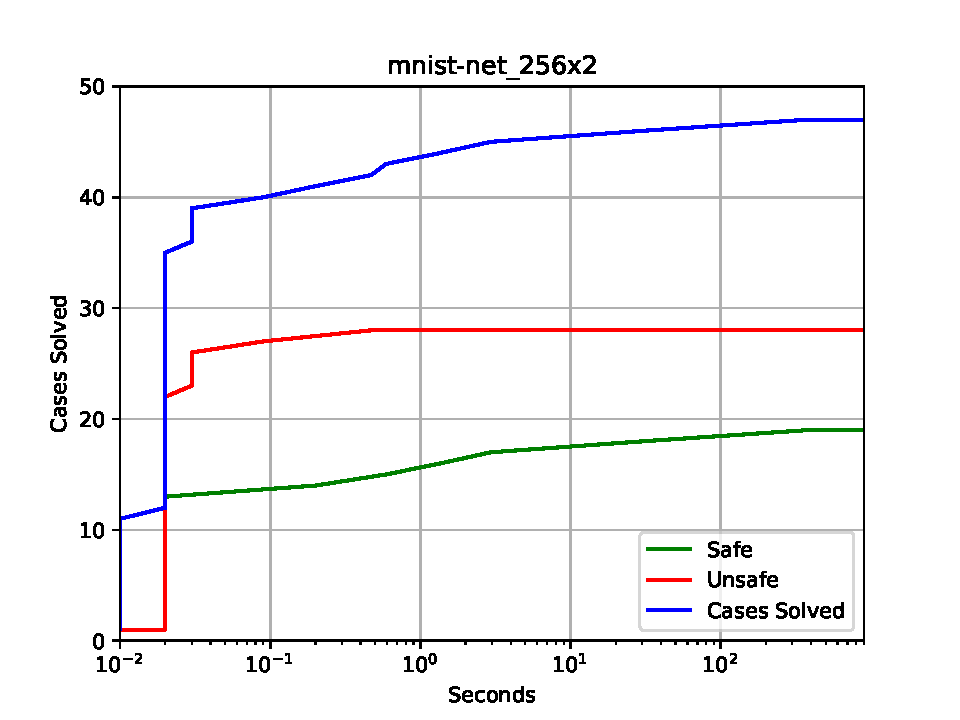
\includegraphics[scale=0.8]{figures/mnist-net_256x2.pdf}
\end{figure}

\begin{figure}[!ht]
\center
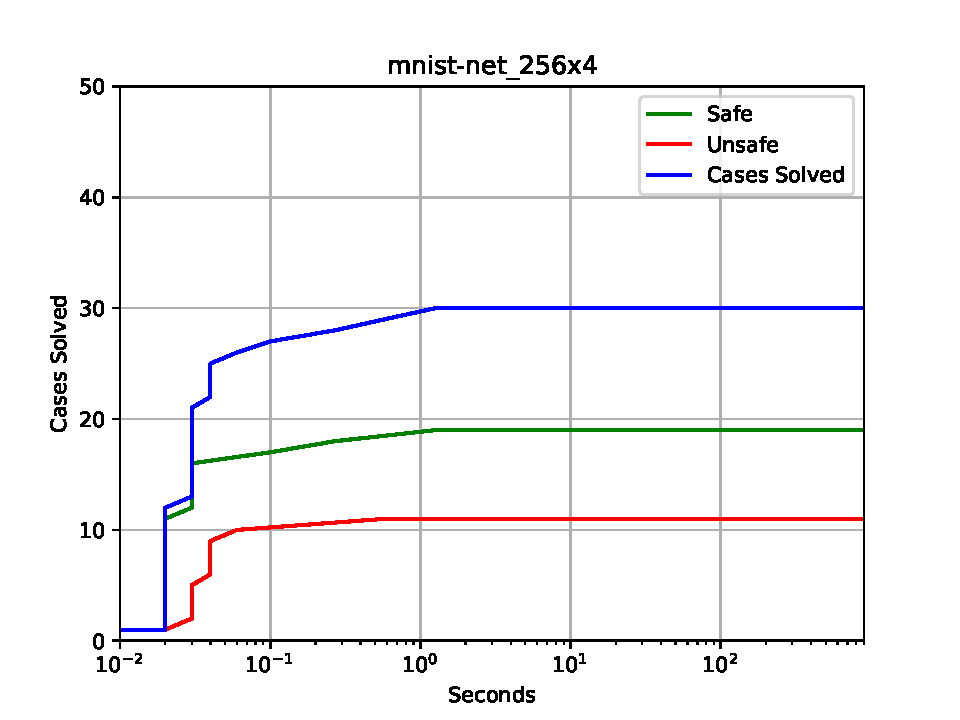
\includegraphics[scale=0.8]{figures/mnist-net_256x4.pdf}
\end{figure}

\begin{figure}[!ht]
\center
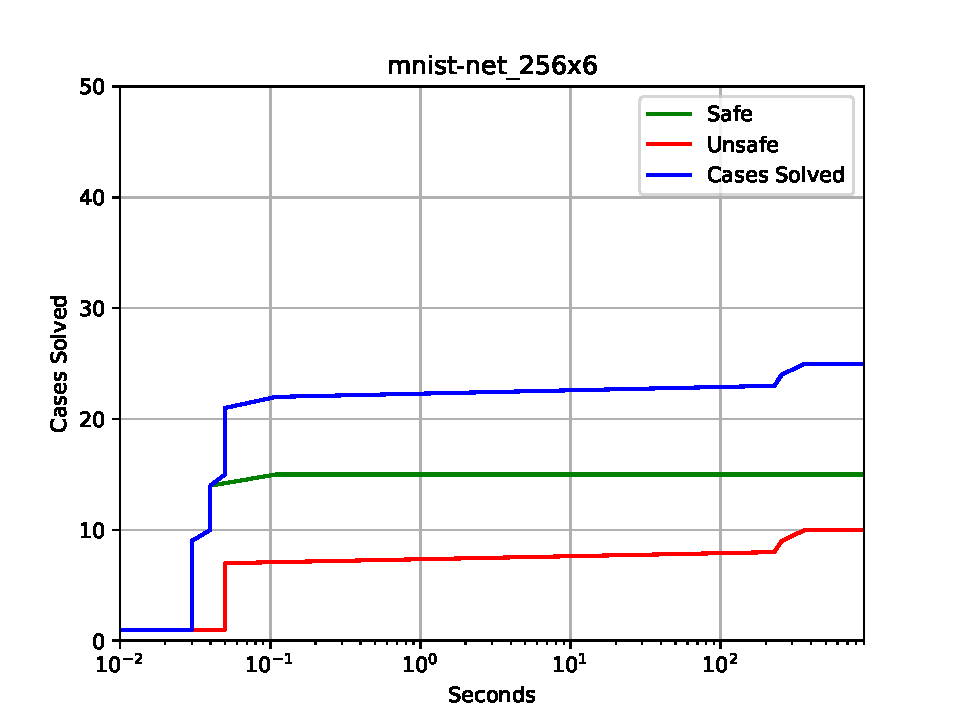
\includegraphics[scale=0.8]{figures/mnist-net_256x6.pdf}
\end{figure}

\begin{figure}[!ht]
\center
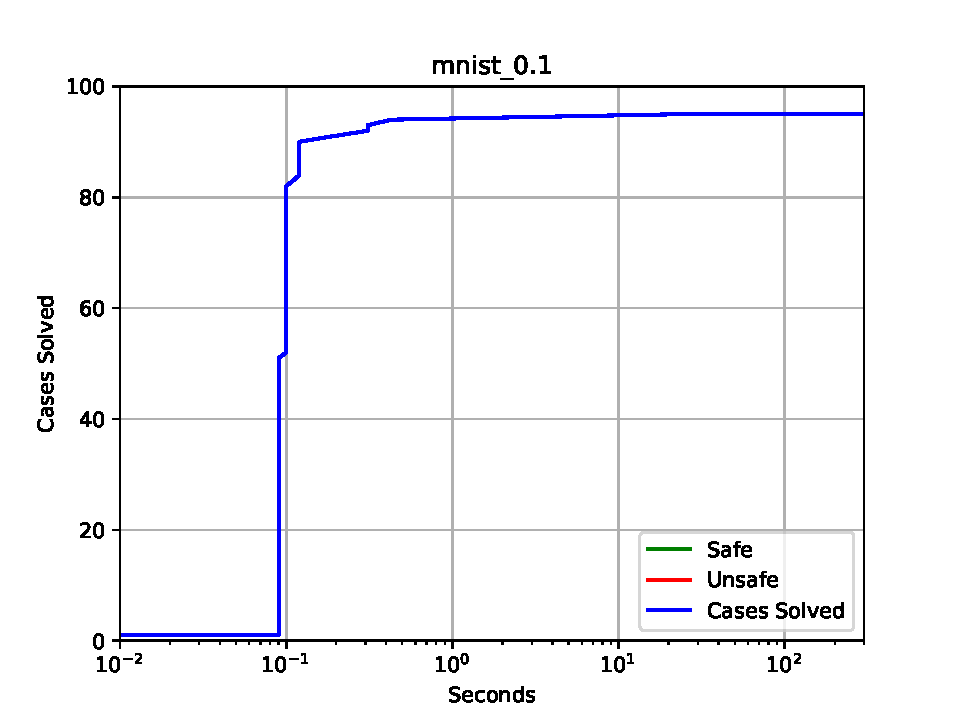
\includegraphics[scale=0.8]{figures/mnist_0.1.pdf}
\end{figure}

\begin{figure}[!ht]
\center
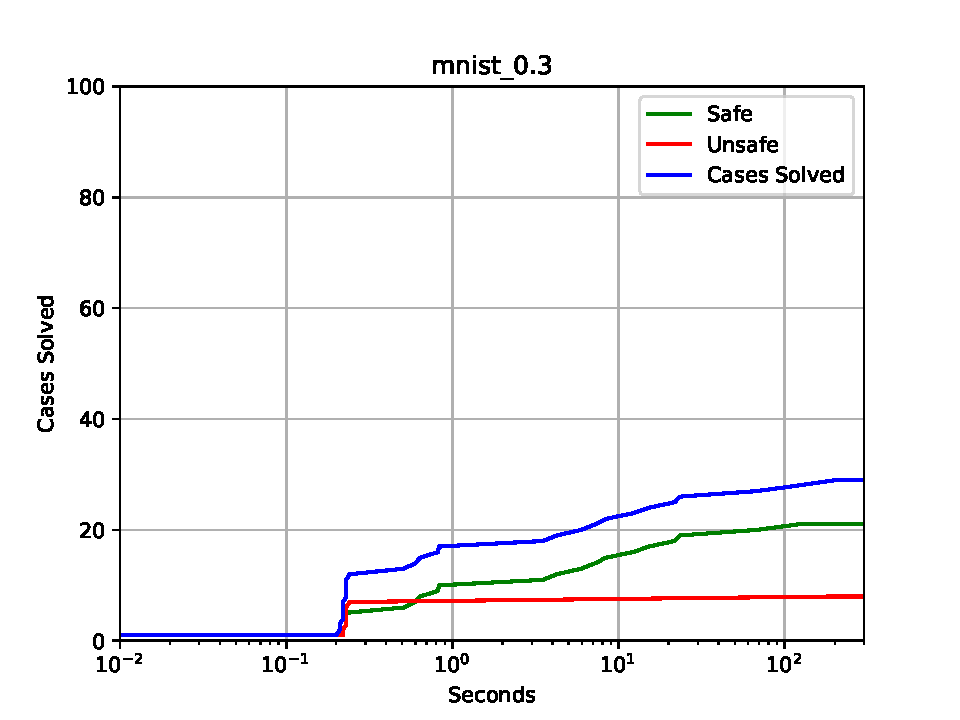
\includegraphics[scale=0.8]{figures/mnist_0.3.pdf}
\end{figure}

\begin{figure}[!ht]
\center
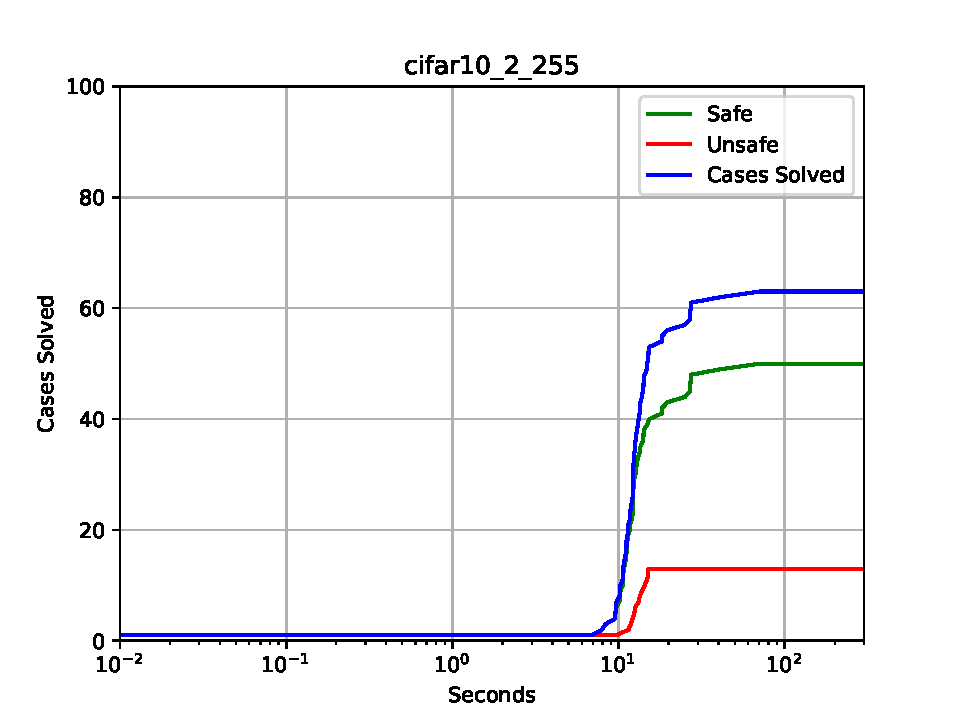
\includegraphics[scale=0.8]{figures/cifar10_2_255.pdf}
\end{figure}

\begin{figure}[!ht]
\center
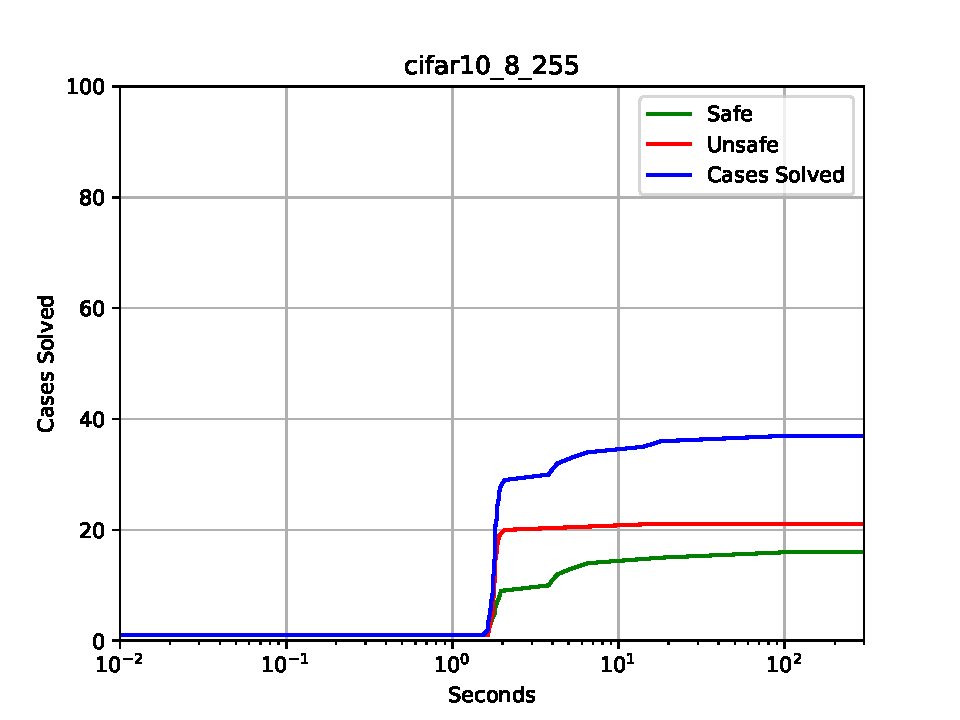
\includegraphics[scale=0.8]{figures/cifar10_8_255.pdf}
\end{figure}

\begin{figure}[!ht]
\center
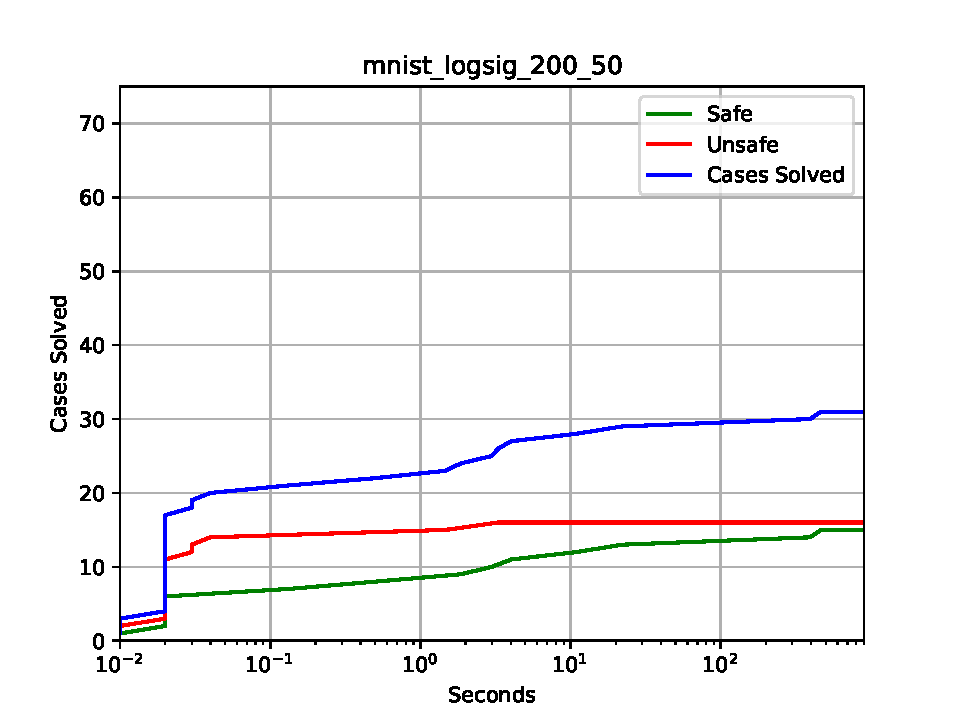
\includegraphics[scale=0.8]{figures/mnist_logsig_200_50.pdf}
\end{figure}

\begin{figure}[!ht]
\center
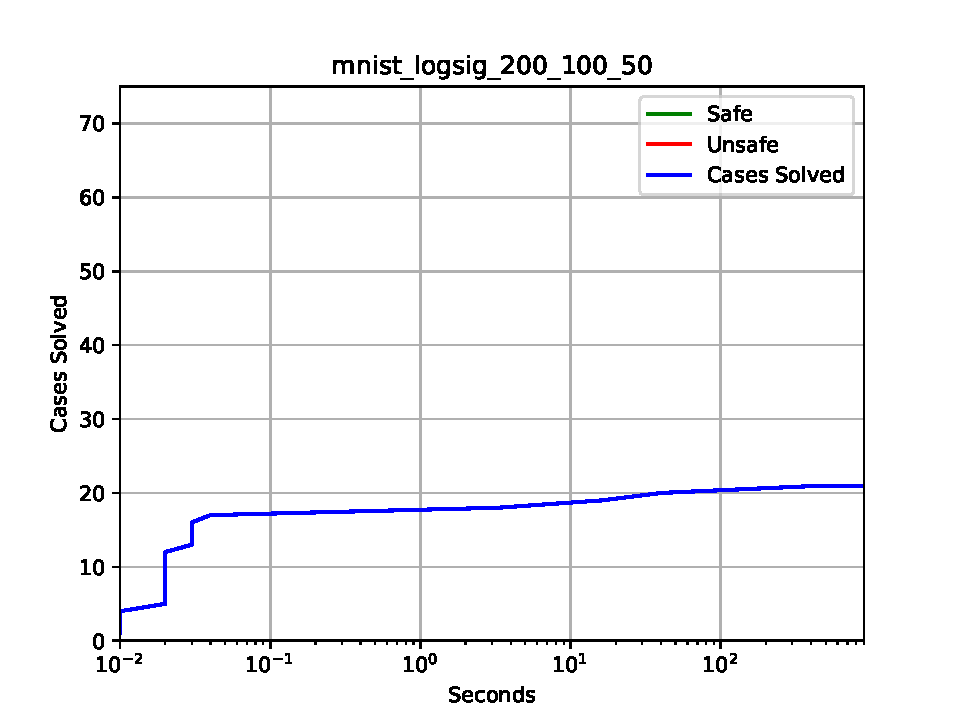
\includegraphics[scale=0.8]{figures/mnist_logsig_200_100_50.pdf}
\end{figure}

\begin{figure}[!ht]
\center
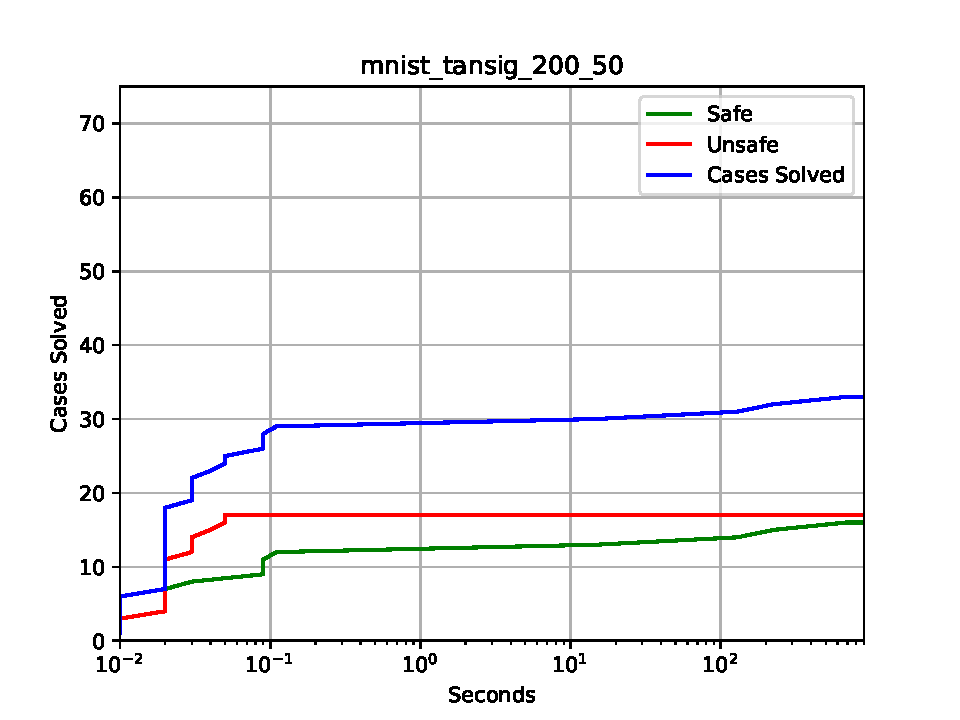
\includegraphics[scale=0.8]{figures/mnist_tansig_200_50.pdf}
\end{figure}

\begin{figure}[!ht]
\center
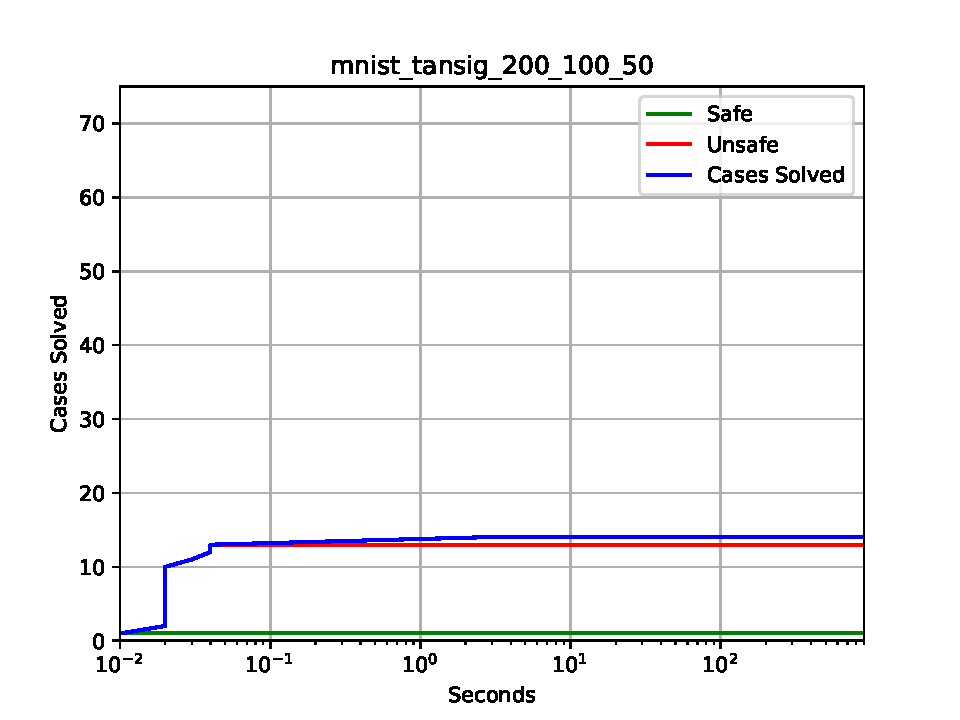
\includegraphics[scale=0.8]{figures/mnist_tansig_200_100_50.pdf}
\end{figure}

\begin{table}[!ht]
  \centering
  \caption{mnist-net 256x2}
  \footnotesize
  \begin{tabular}{|llr|llr|}
    \toprule
    \multicolumn{3}{|c|}{Epsilon: 0.020} & \multicolumn{3}{|c|}{Epsilon: 0.050} \\
    \midrule
    Image & Status & Time(s) &Image & Status & Time(s)\\ 
    \midrule
    0 & Unsafe & 0.09 &    0 & Unsafe & 0.02\\ 
    1 & Safe & 0.01 &    1 & Unsafe & 0.02\\ 
    2 & Unsafe & 0.02 &    2 & Unsafe & 0.02\\ 
    3 & Safe & 0.01 &    3 & Unsafe & 0.02\\ 
    4 & Unsafe & 0.02 &    4 & Unsafe & 0.02\\ 
    5 & Safe & 0.2 &    5 & Unsafe & 0.02\\ 
    6 & Safe & 378.33 &    6 & Unsafe & 0.02\\ 
    7 & Safe & 2.94 &    7 & Unsafe & 0.02\\ 
    8 & Unsafe & 0.02 &    8 & Unsafe & 0.02\\ 
    9 & Safe & 0.01 &    9 & Unsafe & 0.02\\ 
    10 & Safe & 0.01 &    10 & Undecided & 900.0\\ 
    11 & Safe & 0.01 &    11 & Unsafe & 0.03\\ 
    12 & Safe & 0.01 &    12 & Unsafe & 0.02\\ 
    13 & Safe & 0.01 &    13 & Unsafe & 0.02\\ 
    14 & Safe & 0.01 &    14 & Unsafe & 0.47\\ 
    15 & Safe & 0.01 &    15 & Undecided & 900.0\\ 
    16 & Safe & 0.01 &    16 & Unsafe & 0.03\\ 
    17 & Safe & 30.92 &    17 & Unsafe & 0.02\\ 
    18 & Unsafe & 0.03 &    18 & Unsafe & 0.02\\ 
    19 & Safe & 0.59 &    19 & Unsafe & 0.02\\ 
    20 & Safe & 0.02 &    20 & Unsafe & 0.02\\ 
    21 & Safe & 1.36 &    21 & Unsafe & 0.02\\ 
    22 & Safe & 0.02 &    22 & Undecided & 900.0\\ 
    23 & Safe & 0.01 &    23 & Unsafe & 0.03\\ 
    24 & Unsafe & 0.02 &    24 & Unsafe & 0.02\\ 
    \bottomrule
  \end{tabular}
\end{table}


\begin{table}[!ht]
  \centering
  \caption{mnist-net 256x4}
  \footnotesize
  \begin{tabular}{|llr|llr|}
    \toprule
    \multicolumn{3}{|c|}{Epsilon: 0.020} & \multicolumn{3}{|c|}{Epsilon: 0.050} \\
    \midrule
    Image & Status & Time(s) &Image & Status & Time(s)\\ 
    \midrule
    0 & Safe & 0.1 &    0 & Undecided & 900.0\\ 
    1 & Safe & 0.02 &    1 & Undecided & 900.0\\ 
    2 & Undecided & 900.0 &    2 & Unsafe & 0.58\\ 
    3 & Safe & 0.03 &    3 & Undecided & 900.0\\ 
    4 & Safe & 0.02 &    4 & Undecided & 900.0\\ 
    5 & Safe & 0.27 &    5 & Undecided & 900.0\\ 
    6 & Safe & 0.03 &    6 & Unsafe & 0.04\\ 
    7 & Undecided & 900.0 &    7 & Unsafe & 0.03\\ 
    8 & Safe & 1.26 &    8 & Unsafe & 0.03\\ 
    9 & Safe & 0.03 &    9 & Undecided & 900.0\\ 
    10 & Safe & 0.02 &    10 & Undecided & 900.0\\ 
    11 & Safe & 0.02 &    11 & Undecided & 900.0\\ 
    12 & Safe & 0.02 &    12 & Undecided & 900.0\\ 
    13 & Safe & 0.02 &    13 & Undecided & 900.0\\ 
    14 & Safe & 0.02 &    14 & Unsafe & 0.04\\ 
    15 & Safe & 0.02 &    15 & Undecided & 900.0\\ 
    16 & Undecided & 900.0 &    16 & Unsafe & 0.06\\ 
    17 & Safe & 0.03 &    17 & Undecided & 900.0\\ 
    18 & Unsafe & 0.02 &    18 & Unsafe & 0.04\\ 
    19 & Safe & 0.02 &    19 & Unsafe & 0.03\\ 
    20 & Undecided & 900.0 &    20 & Unsafe & 0.03\\ 
    21 & Safe & 0.03 &    21 & Undecided & 900.0\\ 
    22 & Safe & 0.02 &    22 & Undecided & 900.0\\ 
    23 & Safe & 0.02 &    23 & Undecided & 900.0\\ 
    24 & Undecided & 900.0 &    24 & Unsafe & 0.04\\ 
    \bottomrule
  \end{tabular}
\end{table}


\begin{table}[!ht]
  \centering
  \caption{mnist-net 256x6}
  \footnotesize
  \begin{tabular}{|llr|llr|}
    \toprule
    \multicolumn{3}{|c|}{Epsilon: 0.020} & \multicolumn{3}{|c|}{Epsilon: 0.050} \\
    \midrule
    Image & Status & Time(s) &Image & Status & Time(s)\\ 
    \midrule
    0 & Safe & 0.11 &    0 & Unsafe & 363.99\\ 
    1 & Safe & 0.03 &    1 & Undecided & 900.0\\ 
    2 & Undecided & 900.0 &    2 & Unsafe & 0.05\\ 
    3 & Safe & 0.04 &    3 & Undecided & 900.0\\ 
    4 & Safe & 0.03 &    4 & Undecided & 900.0\\ 
    5 & Undecided & 900.0 &    5 & Undecided & 900.0\\ 
    6 & Undecided & 900.0 &    6 & Unsafe & 0.05\\ 
    7 & Undecided & 900.0 &    7 & Unsafe & 254.71\\ 
    8 & Unsafe & 0.05 &    8 & Unsafe & 0.05\\ 
    9 & Safe & 0.03 &    9 & Undecided & 900.0\\ 
    10 & Safe & 0.03 &    10 & Undecided & 900.0\\ 
    11 & Safe & 0.03 &    11 & Unsafe & 0.05\\ 
    12 & Undecided & 900.0 &    12 & Undecided & 900.0\\ 
    13 & Safe & 0.04 &    13 & Undecided & 900.0\\ 
    14 & Safe & 0.03 &    14 & Undecided & 900.0\\ 
    15 & Safe & 0.03 &    15 & Undecided & 900.0\\ 
    16 & Undecided & 900.0 &    16 & Unsafe & 227.87\\ 
    17 & Safe & 0.04 &    17 & Undecided & 900.0\\ 
    18 & Undecided & 900.0 &    18 & Unsafe & 0.05\\ 
    19 & Safe & 0.04 &    19 & Undecided & 900.0\\ 
    20 & Undecided & 900.0 &    20 & Undecided & 900.0\\ 
    21 & Safe & 0.04 &    21 & Undecided & 900.0\\ 
    22 & Safe & 0.03 &    22 & Undecided & 900.0\\ 
    23 & Safe & 0.03 &    23 & Undecided & 900.0\\ 
    24 & Undecided & 900.0 &    24 & Unsafe & 0.05\\ 
    \bottomrule
  \end{tabular}
\end{table}


\begin{table}[!ht]
  \centering
  \caption{mnist 0.1}
  \footnotesize
  \begin{tabular}{|llr|llr|}
    \toprule
    \multicolumn{3}{|c|}{Epsilon: 0.100} & \multicolumn{3}{|c|}{Epsilon: 0.100} \\
    \midrule
    Image & Status & Time(s) &Image & Status & Time(s)\\ 
    \midrule
    0 & Safe & 0.19 &    50 & Safe & 0.1\\ 
    1 & Safe & 0.1 &    51 & Safe & 0.09\\ 
    2 & Safe & 0.1 &    52 & Safe & 0.1\\ 
    3 & Safe & 0.1 &    53 & Safe & 0.09\\ 
    4 & Safe & 0.1 &    54 & Safe & 0.1\\ 
    5 & Safe & 0.09 &    55 & Safe & 0.1\\ 
    6 & Undecided & 300.0 &    56 & Safe & 0.09\\ 
    7 & Safe & 0.12 &    57 & Safe & 0.1\\ 
    8 & Undecided & 300.0 &    58 & Safe & 0.1\\ 
    9 & Safe & 0.12 &    59 & Safe & 0.43\\ 
    10 & Safe & 0.09 &    60 & Safe & 0.12\\ 
    11 & Safe & 0.09 &    61 & Safe & 0.09\\ 
    12 & Safe & 0.09 &    62 & Undecided & 300.0\\ 
    13 & Safe & 0.09 &    63 & Safe & 0.12\\ 
    14 & Safe & 0.09 &    64 & Safe & 0.1\\ 
    15 & Safe & 0.09 &    65 & Safe & 24.58\\ 
    16 & Safe & 0.09 &    66 & Safe & 0.12\\ 
    17 & Safe & 0.09 &    67 & Safe & 0.09\\ 
    18 & Undecided & 300.0 &    68 & Safe & 0.1\\ 
    19 & Safe & 0.12 &    69 & Safe & 0.09\\ 
    20 & Safe & 0.09 &    70 & Safe & 0.1\\ 
    21 & Safe & 0.09 &    71 & Safe & 0.09\\ 
    22 & Safe & 0.09 &    72 & Safe & 0.1\\ 
    23 & Safe & 0.1 &    73 & Safe & 0.09\\ 
    24 & Safe & 0.1 &    74 & Safe & 0.09\\ 
    25 & Safe & 0.09 &    75 & Safe & 0.09\\ 
    26 & Safe & 0.09 &    76 & Safe & 0.09\\ 
    27 & Safe & 0.09 &    77 & Safe & 0.09\\ 
    28 & Safe & 0.09 &    78 & Safe & 0.1\\ 
    29 & Safe & 0.09 &    79 & Safe & 0.09\\ 
    30 & Safe & 0.09 &    80 & Safe & 0.1\\ 
    31 & Safe & 0.09 &    81 & Safe & 0.09\\ 
    32 & Safe & 0.09 &    82 & Safe & 0.09\\ 
    33 & Safe & 0.1 &    83 & Safe & 0.09\\ 
    34 & Safe & 0.09 &    84 & Safe & 0.1\\ 
    35 & Safe & 0.1 &    85 & Safe & 0.1\\ 
    36 & Safe & 0.09 &    86 & Safe & 0.1\\ 
    37 & Safe & 0.09 &    87 & Safe & 0.09\\ 
    38 & Safe & 0.1 &    88 & Safe & 0.1\\ 
    39 & Safe & 0.09 &    89 & Safe & 0.09\\ 
    40 & Safe & 0.1 &    90 & Safe & 0.1\\ 
    41 & Safe & 0.09 &    91 & Safe & 0.09\\ 
    42 & Safe & 0.09 &    92 & Undecided & 300.0\\ 
    43 & Safe & 0.09 &    93 & Safe & 0.31\\ 
    44 & Safe & 0.09 &    94 & Safe & 0.11\\ 
    45 & Safe & 0.09 &    95 & Safe & 0.31\\ 
    46 & Safe & 0.09 &    96 & Safe & 0.12\\ 
    47 & Safe & 0.1 &    97 & Safe & 0.09\\ 
    48 & Safe & 0.1 &    98 & Safe & 0.1\\ 
    49 & Safe & 0.1 &    99 & Safe & 0.09\\ 
    \bottomrule
  \end{tabular}
\end{table}


\begin{table}[!ht]
  \centering
  \caption{mnist 0.3}
  \footnotesize
  \begin{tabular}{|llr|llr|}
    \toprule
    \multicolumn{3}{|c|}{Epsilon: 0.300} & \multicolumn{3}{|c|}{Epsilon: 0.300} \\
    \midrule
    Image & Status & Time(s) &Image & Status & Time(s)\\ 
    \midrule
    0 & Safe & 12.23 &    50 & Undecided & 300.0\\ 
    1 & Undecided & 300.0 &    51 & Undecided & 300.0\\ 
    2 & Undecided & 300.0 &    52 & Undecided & 300.0\\ 
    3 & Undecided & 300.0 &    53 & Undecided & 300.0\\ 
    4 & Undecided & 300.0 &    54 & Undecided & 300.0\\ 
    5 & Safe & 21.79 &    55 & Safe & 15.22\\ 
    6 & Undecided & 300.0 &    56 & Undecided & 300.0\\ 
    7 & Undecided & 300.0 &    57 & Undecided & 300.0\\ 
    8 & Unsafe & 0.22 &    58 & Undecided & 300.0\\ 
    9 & Undecided & 300.0 &    59 & Undecided & 300.0\\ 
    10 & Safe & 23.35 &    60 & Safe & 0.22\\ 
    11 & Undecided & 300.0 &    61 & Undecided & 300.0\\ 
    12 & Undecided & 300.0 &    62 & Unsafe & 204.86\\ 
    13 & Undecided & 300.0 &    63 & Unsafe & 0.23\\ 
    14 & Safe & 0.2 &    64 & Undecided & 300.0\\ 
    15 & Undecided & 300.0 &    65 & Misclassified & 0.0\\ 
    16 & Undecided & 300.0 &    66 & Undecided & 300.0\\ 
    17 & Safe & 5.95 &    67 & Undecided & 300.0\\ 
    18 & Unsafe & 0.24 &    68 & Undecided & 300.0\\ 
    19 & Undecided & 300.0 &    69 & Undecided & 300.0\\ 
    20 & Undecided & 300.0 &    70 & Safe & 0.22\\ 
    21 & Undecided & 300.0 &    71 & Safe & 7.25\\ 
    22 & Undecided & 300.0 &    72 & Undecided & 300.0\\ 
    23 & Undecided & 300.0 &    73 & Unsafe & 0.22\\ 
    24 & Undecided & 300.0 &    74 & Safe & 0.6\\ 
    25 & Safe & 8.41 &    75 & Undecided & 300.0\\ 
    26 & Undecided & 300.0 &    76 & Undecided & 300.0\\ 
    27 & Undecided & 300.0 &    77 & Undecided & 300.0\\ 
    28 & Undecided & 300.0 &    78 & Undecided & 300.0\\ 
    29 & Undecided & 300.0 &    79 & Safe & 0.83\\ 
    30 & Undecided & 300.0 &    80 & Undecided & 300.0\\ 
    31 & Undecided & 300.0 &    81 & Undecided & 300.0\\ 
    32 & Safe & 4.25 &    82 & Safe & 0.82\\ 
    33 & Unsafe & 0.23 &    83 & Safe & 120.14\\ 
    34 & Undecided & 300.0 &    84 & Undecided & 300.0\\ 
    35 & Undecided & 300.0 &    85 & Safe & 3.52\\ 
    36 & Undecided & 300.0 &    86 & Undecided & 300.0\\ 
    37 & Safe & 0.21 &    87 & Undecided & 300.0\\ 
    38 & Undecided & 300.0 &    88 & Undecided & 300.0\\ 
    39 & Safe & 0.21 &    89 & Undecided & 300.0\\ 
    40 & Safe & 0.51 &    90 & Undecided & 300.0\\ 
    41 & Undecided & 300.0 &    91 & Undecided & 300.0\\ 
    42 & Undecided & 300.0 &    92 & Unsafe & 0.23\\ 
    43 & Unsafe & 0.23 &    93 & Undecided & 300.0\\ 
    44 & Undecided & 300.0 &    94 & Safe & 67.79\\ 
    45 & Undecided & 300.0 &    95 & Undecided & 300.0\\ 
    46 & Safe & 0.64 &    96 & Undecided & 300.0\\ 
    47 & Undecided & 300.0 &    97 & Undecided & 300.0\\ 
    48 & Undecided & 300.0 &    98 & Undecided & 300.0\\ 
    49 & Undecided & 300.0 &    99 & Undecided & 300.0\\ 
    \bottomrule
  \end{tabular}
\end{table}


\begin{table}[!ht]
  \centering
  \caption{cifar10 2 255}
  \footnotesize
  \begin{tabular}{|llr|llr|}
    \toprule
    \multicolumn{3}{|c|}{Epsilon: 0.008} & \multicolumn{3}{|c|}{Epsilon: 0.008} \\
    \midrule
    Image & Status & Time(s) &Image & Status & Time(s)\\ 
    \midrule
    0 & Unsafe & 9.7 &    50 & Undecided & 300.0\\ 
    1 & Safe & 7.96 &    51 & Undecided & 300.0\\ 
    2 & Undecided & 300.0 &    52 & Misclassified & 0.0\\ 
    3 & Safe & 18.21 &    53 & Undecided & 300.0\\ 
    4 & Undecided & 300.0 &    54 & Safe & 10.8\\ 
    5 & Safe & 71.23 &    55 & Safe & 10.65\\ 
    6 & Safe & 19.63 &    56 & Misclassified & 0.0\\ 
    7 & Misclassified & 0.0 &    57 & Misclassified & 0.0\\ 
    8 & Undecided & 300.0 &    58 & Misclassified & 0.0\\ 
    9 & Undecided & 300.0 &    59 & Misclassified & 0.0\\ 
    10 & Safe & 15.32 &    60 & Safe & 13.06\\ 
    11 & Safe & 9.65 &    61 & Misclassified & 0.0\\ 
    12 & Unsafe & 13.84 &    62 & Safe & 11.31\\ 
    13 & Safe & 12.19 &    63 & Misclassified & 0.0\\ 
    14 & Safe & 13.4 &    64 & Undecided & 300.0\\ 
    15 & Safe & 12.28 &    65 & Unsafe & 13.41\\ 
    16 & Undecided & 300.0 &    66 & Undecided & 300.0\\ 
    17 & Safe & 13.54 &    67 & Safe & 10.12\\ 
    18 & Safe & 11.43 &    68 & Undecided & 300.0\\ 
    19 & Safe & 14.13 &    69 & Misclassified & 0.0\\ 
    20 & Safe & 25.12 &    70 & Misclassified & 0.0\\ 
    21 & Safe & 6.88 &    71 & Undecided & 300.0\\ 
    22 & Misclassified & 0.0 &    72 & Safe & 9.58\\ 
    23 & Safe & 12.76 &    73 & Safe & 12.03\\ 
    24 & Misclassified & 0.0 &    74 & Unsafe & 12.18\\ 
    25 & Undecided & 300.0 &    75 & Safe & 11.16\\ 
    26 & Unsafe & 15.14 &    76 & Unsafe & 12.46\\ 
    27 & Undecided & 300.0 &    77 & Undecided & 300.0\\ 
    28 & Unsafe & 12.58 &    78 & Safe & 27.22\\ 
    29 & Safe & 14.16 &    79 & Safe & 9.53\\ 
    30 & Undecided & 300.0 &    80 & Safe & 11.73\\ 
    31 & Unsafe & 14.35 &    81 & Safe & 10.26\\ 
    32 & Unsafe & 14.85 &    82 & Safe & 12.22\\ 
    33 & Undecided & 300.0 &    83 & Safe & 10.25\\ 
    34 & Safe & 12.41 &    84 & Safe & 10.59\\ 
    35 & Misclassified & 0.0 &    85 & Misclassified & 0.0\\ 
    36 & Unsafe & 15.12 &    86 & Unsafe & 11.85\\ 
    37 & Unsafe & 11.47 &    87 & Misclassified & 0.0\\ 
    38 & Safe & 12.91 &    88 & Safe & 11.72\\ 
    39 & Safe & 41.37 &    89 & Safe & 12.22\\ 
    40 & Safe & 12.64 &    90 & Safe & 11.15\\ 
    41 & Safe & 12.31 &    91 & Misclassified & 0.0\\ 
    42 & Undecided & 300.0 &    92 & Safe & 10.91\\ 
    43 & Safe & 14.87 &    93 & Safe & 26.9\\ 
    44 & Safe & 10.62 &    94 & Safe & 26.94\\ 
    45 & Safe & 11.16 &    95 & Unsafe & 13.2\\ 
    46 & Safe & 27.41 &    96 & Safe & 13.98\\ 
    47 & Misclassified & 0.0 &    97 & Safe & 18.3\\ 
    48 & Undecided & 300.0 &    98 & Safe & 8.34\\ 
    49 & Misclassified & 0.0 &    99 & Safe & 12.21\\ 
    \bottomrule
  \end{tabular}
\end{table}


\begin{table}[!ht]
  \centering
  \caption{cifar10 8 255}
  \footnotesize
  \begin{tabular}{|llr|llr|}
    \toprule
    \multicolumn{3}{|c|}{Epsilon: 0.031} & \multicolumn{3}{|c|}{Epsilon: 0.031} \\
    \midrule
    Image & Status & Time(s) &Image & Status & Time(s)\\ 
    \midrule
    0 & Misclassified & 0.0 &    50 & Safe & 1.96\\ 
    1 & Safe & 6.53 &    51 & Undecided & 300.0\\ 
    2 & Undecided & 300.0 &    52 & Misclassified & 0.0\\ 
    3 & Misclassified & 0.0 &    53 & Misclassified & 0.0\\ 
    4 & Unsafe & 1.85 &    54 & Safe & 4.01\\ 
    5 & Undecided & 300.0 &    55 & Safe & 105.64\\ 
    6 & Misclassified & 0.0 &    56 & Misclassified & 0.0\\ 
    7 & Misclassified & 0.0 &    57 & Misclassified & 0.0\\ 
    8 & Misclassified & 0.0 &    58 & Misclassified & 0.0\\ 
    9 & Unsafe & 1.77 &    59 & Misclassified & 0.0\\ 
    10 & Undecided & 300.0 &    60 & Unsafe & 1.81\\ 
    11 & Undecided & 300.0 &    61 & Misclassified & 0.0\\ 
    12 & Misclassified & 0.0 &    62 & Misclassified & 0.0\\ 
    13 & Safe & 5.19 &    63 & Misclassified & 0.0\\ 
    14 & Undecided & 300.0 &    64 & Undecided & 300.0\\ 
    15 & Undecided & 300.0 &    65 & Misclassified & 0.0\\ 
    16 & Safe & 1.8 &    66 & Undecided & 300.0\\ 
    17 & Misclassified & 0.0 &    67 & Unsafe & 1.78\\ 
    18 & Safe & 1.74 &    68 & Misclassified & 0.0\\ 
    19 & Unsafe & 1.88 &    69 & Misclassified & 0.0\\ 
    20 & Misclassified & 0.0 &    70 & Misclassified & 0.0\\ 
    21 & Safe & 1.53 &    71 & Undecided & 300.0\\ 
    22 & Misclassified & 0.0 &    72 & Undecided & 300.0\\ 
    23 & Unsafe & 1.81 &    73 & Undecided & 300.0\\ 
    24 & Misclassified & 0.0 &    74 & Unsafe & 1.92\\ 
    25 & Misclassified & 0.0 &    75 & Misclassified & 0.0\\ 
    26 & Misclassified & 0.0 &    76 & Undecided & 300.0\\ 
    27 & Misclassified & 0.0 &    77 & Misclassified & 0.0\\ 
    28 & Undecided & 300.0 &    78 & Misclassified & 0.0\\ 
    29 & Safe & 3.8 &    79 & Unsafe & 1.64\\ 
    30 & Unsafe & 2.06 &    80 & Undecided & 300.0\\ 
    31 & Misclassified & 0.0 &    81 & Safe & 1.86\\ 
    32 & Unsafe & 1.75 &    82 & Safe & 1.81\\ 
    33 & Unsafe & 1.8 &    83 & Unsafe & 1.66\\ 
    34 & Safe & 4.3 &    84 & Undecided & 300.0\\ 
    35 & Misclassified & 0.0 &    85 & Misclassified & 0.0\\ 
    36 & Misclassified & 0.0 &    86 & Unsafe & 1.86\\ 
    37 & Misclassified & 0.0 &    87 & Misclassified & 0.0\\ 
    38 & Unsafe & 1.82 &    88 & Undecided & 300.0\\ 
    39 & Unsafe & 1.78 &    89 & Unsafe & 1.8\\ 
    40 & Misclassified & 0.0 &    90 & Unsafe & 1.75\\ 
    41 & Safe & 1.92 &    91 & Misclassified & 0.0\\ 
    42 & Misclassified & 0.0 &    92 & Safe & 1.7\\ 
    43 & Misclassified & 0.0 &    93 & Misclassified & 0.0\\ 
    44 & Unsafe & 1.69 &    94 & Misclassified & 0.0\\ 
    45 & Undecided & 300.0 &    95 & Unsafe & 1.75\\ 
    46 & Misclassified & 0.0 &    96 & Unsafe & 14.08\\ 
    47 & Misclassified & 0.0 &    97 & Undecided & 300.0\\ 
    48 & Misclassified & 0.0 &    98 & Safe & 1.64\\ 
    49 & Safe & 18.1 &    99 & Unsafe & 1.71\\ 
    \bottomrule
  \end{tabular}
\end{table}


\begin{table}[!ht]
  \centering
  \caption{mnist logsig 200 50}
  \footnotesize
  \begin{tabular}{|llr|llr|llr|}
    \toprule
    \multicolumn{3}{|c|}{Epsilon: 3.000} & \multicolumn{3}{|c|}{Epsilon: 5.000} & \multicolumn{3}{|c|}{Epsilon: 12.000} \\
    \midrule
    Image & Status & Time(s) &Image & Status & Time(s) &Image & Status & Time(s)\\ 
    \midrule
    0 & Safe & 0.13 &    0 & Undecided & 900.0 &    0 & Undecided & 900.0\\ 
    1 & Safe & 4.03 &    1 & Undecided & 900.0 &    1 & Undecided & 900.0\\ 
    2 & Undecided & 900.0 &    2 & Undecided & 900.0 &    2 & Unsafe & 0.03\\ 
    3 & Safe & 0.02 &    3 & Safe & 464.32 &    3 & Undecided & 900.0\\ 
    4 & Safe & 22.06 &    4 & Undecided & 900.0 &    4 & Unsafe & 0.03\\ 
    5 & Safe & 0.02 &    5 & Undecided & 900.0 &    5 & Undecided & 900.0\\ 
    6 & Undecided & 900.0 &    6 & Undecided & 900.0 &    6 & Unsafe & 0.02\\ 
    7 & Undecided & 900.0 &    7 & Undecided & 900.0 &    7 & Undecided & 900.0\\ 
    8 & Unsafe & 0.02 &    8 & Unsafe & 0.02 &    8 & Unsafe & 0.02\\ 
    9 & Safe & 2.99 &    9 & Undecided & 900.0 &    9 & Unsafe & 0.01\\ 
    10 & Safe & 0.02 &    10 & Undecided & 900.0 &    10 & Undecided & 900.0\\ 
    11 & Undecided & 900.0 &    11 & Undecided & 900.0 &    11 & Unsafe & 0.04\\ 
    12 & Safe & 10.91 &    12 & Undecided & 900.0 &    12 & Undecided & 900.0\\ 
    13 & Safe & 0.02 &    13 & Undecided & 900.0 &    13 & Undecided & 900.0\\ 
    14 & Safe & 0.01 &    14 & Undecided & 900.0 &    14 & Undecided & 900.0\\ 
    15 & Undecided & 900.0 &    15 & Undecided & 900.0 &    15 & Unsafe & 0.02\\ 
    16 & Undecided & 900.0 &    16 & Undecided & 900.0 &    16 & Unsafe & 3.3\\ 
    17 & Safe & 0.02 &    17 & Undecided & 900.0 &    17 & Undecided & 900.0\\ 
    18 & Unsafe & 0.01 &    18 & Unsafe & 0.02 &    18 & Unsafe & 0.02\\ 
    19 & Safe & 0.5 &    19 & Undecided & 900.0 &    19 & Undecided & 900.0\\ 
    20 & Safe & 1.86 &    20 & Undecided & 900.0 &    20 & Unsafe & 0.02\\ 
    21 & Undecided & 900.0 &    21 & Undecided & 900.0 &    21 & Unsafe & 1.47\\ 
    22 & Safe & 394.82 &    22 & Undecided & 900.0 &    22 & Undecided & 900.0\\ 
    23 & Undecided & 900.0 &    23 & Undecided & 900.0 &    23 & Undecided & 900.0\\ 
    24 & Undecided & 900.0 &    24 & Undecided & 900.0 &    24 & Unsafe & 0.02\\ 
    \bottomrule
  \end{tabular}
\end{table}


\begin{table}[!ht]
  \centering
  \caption{mnist logsig 200 100 50}
  \footnotesize
  \begin{tabular}{|llr|llr|llr|}
    \toprule
    \multicolumn{3}{|c|}{Epsilon: 3.000} & \multicolumn{3}{|c|}{Epsilon: 5.000} & \multicolumn{3}{|c|}{Epsilon: 12.000} \\
    \midrule
    Image & Status & Time(s) &Image & Status & Time(s) &Image & Status & Time(s)\\ 
    \midrule
    0 & Undecided & 900.0 &    0 & Undecided & 900.0 &    0 & Undecided & 900.0\\ 
    1 & Undecided & 900.0 &    1 & Undecided & 900.0 &    1 & Undecided & 900.0\\ 
    2 & Undecided & 900.0 &    2 & Undecided & 900.0 &    2 & Unsafe & 0.03\\ 
    3 & Undecided & 900.0 &    3 & Undecided & 900.0 &    3 & Undecided & 900.0\\ 
    4 & Undecided & 900.0 &    4 & Undecided & 900.0 &    4 & Unsafe & 0.02\\ 
    5 & Undecided & 900.0 &    5 & Undecided & 900.0 &    5 & Unsafe & 0.02\\ 
    6 & Undecided & 900.0 &    6 & Undecided & 900.0 &    6 & Unsafe & 0.01\\ 
    7 & Undecided & 900.0 &    7 & Undecided & 900.0 &    7 & Unsafe & 0.02\\ 
    8 & Unsafe & 3.29 &    8 & Unsafe & 0.03 &    8 & Unsafe & 0.01\\ 
    9 & Undecided & 900.0 &    9 & Undecided & 900.0 &    9 & Unsafe & 484.32\\ 
    10 & Undecided & 900.0 &    10 & Undecided & 900.0 &    10 & Unsafe & 16.27\\ 
    11 & Undecided & 900.0 &    11 & Undecided & 900.0 &    11 & Unsafe & 0.03\\ 
    12 & Undecided & 900.0 &    12 & Undecided & 900.0 &    12 & Unsafe & 0.01\\ 
    13 & Undecided & 900.0 &    13 & Undecided & 900.0 &    13 & Undecided & 900.0\\ 
    14 & Undecided & 900.0 &    14 & Undecided & 900.0 &    14 & Undecided & 900.0\\ 
    15 & Undecided & 900.0 &    15 & Undecided & 900.0 &    15 & Unsafe & 0.03\\ 
    16 & Undecided & 900.0 &    16 & Undecided & 900.0 &    16 & Unsafe & 40.09\\ 
    17 & Undecided & 900.0 &    17 & Undecided & 900.0 &    17 & Undecided & 900.0\\ 
    18 & Unsafe & 0.02 &    18 & Unsafe & 0.02 &    18 & Unsafe & 0.02\\ 
    19 & Undecided & 900.0 &    19 & Undecided & 900.0 &    19 & Unsafe & 0.02\\ 
    20 & Undecided & 900.0 &    20 & Unsafe & 0.04 &    20 & Unsafe & 0.01\\ 
    21 & Undecided & 900.0 &    21 & Undecided & 900.0 &    21 & Undecided & 900.0\\ 
    22 & Undecided & 900.0 &    22 & Undecided & 900.0 &    22 & Undecided & 900.0\\ 
    23 & Undecided & 900.0 &    23 & Undecided & 900.0 &    23 & Undecided & 900.0\\ 
    24 & Undecided & 900.0 &    24 & Undecided & 900.0 &    24 & Unsafe & 0.02\\ 
    \bottomrule
  \end{tabular}
\end{table}


\begin{table}[!ht]
  \centering
  \caption{mnist tansig 200 50}
  \footnotesize
  \begin{tabular}{|llr|llr|llr|}
    \toprule
    \multicolumn{3}{|c|}{Epsilon: 3.000} & \multicolumn{3}{|c|}{Epsilon: 5.000} & \multicolumn{3}{|c|}{Epsilon: 12.000} \\
    \midrule
    Image & Status & Time(s) &Image & Status & Time(s) &Image & Status & Time(s)\\ 
    \midrule
    0 & Safe & 0.09 &    0 & Undecided & 900.0 &    0 & Undecided & 900.0\\ 
    1 & Safe & 0.01 &    1 & Undecided & 900.0 &    1 & Undecided & 900.0\\ 
    2 & Undecided & 900.0 &    2 & Undecided & 900.0 &    2 & Unsafe & 0.02\\ 
    3 & Safe & 0.11 &    3 & Undecided & 900.0 &    3 & Undecided & 900.0\\ 
    4 & Undecided & 900.0 &    4 & Undecided & 900.0 &    4 & Unsafe & 0.03\\ 
    5 & Undecided & 900.0 &    5 & Undecided & 900.0 &    5 & Unsafe & 0.04\\ 
    6 & Safe & 224.27 &    6 & Undecided & 900.0 &    6 & Unsafe & 0.02\\ 
    7 & Safe & 0.02 &    7 & Undecided & 900.0 &    7 & Undecided & 900.0\\ 
    8 & Unsafe & 0.01 &    8 & Unsafe & 0.02 &    8 & Unsafe & 0.02\\ 
    9 & Safe & 683.25 &    9 & Undecided & 900.0 &    9 & Unsafe & 0.05\\ 
    10 & Safe & 14.84 &    10 & Undecided & 900.0 &    10 & Unsafe & 0.01\\ 
    11 & Safe & 0.09 &    11 & Undecided & 900.0 &    11 & Unsafe & 0.03\\ 
    12 & Safe & 0.02 &    12 & Undecided & 900.0 &    12 & Undecided & 900.0\\ 
    13 & Safe & 0.01 &    13 & Undecided & 900.0 &    13 & Undecided & 900.0\\ 
    14 & Safe & 0.09 &    14 & Undecided & 900.0 &    14 & Undecided & 900.0\\ 
    15 & Undecided & 900.0 &    15 & Unsafe & 0.02 &    15 & Unsafe & 0.02\\ 
    16 & Safe & 129.39 &    16 & Undecided & 900.0 &    16 & Undecided & 900.0\\ 
    17 & Safe & 0.02 &    17 & Undecided & 900.0 &    17 & Undecided & 900.0\\ 
    18 & Undecided & 900.0 &    18 & Unsafe & 0.02 &    18 & Unsafe & 0.02\\ 
    19 & Safe & 0.02 &    19 & Undecided & 900.0 &    19 & Undecided & 900.0\\ 
    20 & Undecided & 900.0 &    20 & Undecided & 900.0 &    20 & Unsafe & 0.05\\ 
    21 & Undecided & 900.0 &    21 & Undecided & 900.0 &    21 & Unsafe & 0.01\\ 
    22 & Safe & 0.03 &    22 & Undecided & 900.0 &    22 & Undecided & 900.0\\ 
    23 & Safe & 0.01 &    23 & Undecided & 900.0 &    23 & Undecided & 900.0\\ 
    24 & Undecided & 900.0 &    24 & Undecided & 900.0 &    24 & Unsafe & 0.03\\ 
    \bottomrule
  \end{tabular}
\end{table}


\begin{table}[!ht]
  \centering
  \caption{mnist tansig 200 100 50}
  \footnotesize
  \begin{tabular}{|llr|llr|llr|}
    \toprule
    \multicolumn{3}{|c|}{Epsilon: 3.000} & \multicolumn{3}{|c|}{Epsilon: 5.000} & \multicolumn{3}{|c|}{Epsilon: 12.000} \\
    \midrule
    Image & Status & Time(s) &Image & Status & Time(s) &Image & Status & Time(s)\\ 
    \midrule
    0 & Undecided & 900.0 &    0 & Undecided & 900.0 &    0 & Undecided & 900.0\\ 
    1 & Undecided & 900.0 &    1 & Undecided & 900.0 &    1 & Undecided & 900.0\\ 
    2 & Undecided & 900.0 &    2 & Undecided & 900.0 &    2 & Unsafe & 0.02\\ 
    3 & Undecided & 900.0 &    3 & Undecided & 900.0 &    3 & Undecided & 900.0\\ 
    4 & Undecided & 900.0 &    4 & Undecided & 900.0 &    4 & Unsafe & 0.04\\ 
    5 & Undecided & 900.0 &    5 & Undecided & 900.0 &    5 & Unsafe & 0.02\\ 
    6 & Undecided & 900.0 &    6 & Undecided & 900.0 &    6 & Unsafe & 0.02\\ 
    7 & Undecided & 900.0 &    7 & Undecided & 900.0 &    7 & Unsafe & 0.02\\ 
    8 & Unsafe & 0.02 &    8 & Unsafe & 0.02 &    8 & Unsafe & 0.01\\ 
    9 & Undecided & 900.0 &    9 & Undecided & 900.0 &    9 & Unsafe & 0.04\\ 
    10 & Undecided & 900.0 &    10 & Undecided & 900.0 &    10 & Undecided & 900.0\\ 
    11 & Undecided & 900.0 &    11 & Undecided & 900.0 &    11 & Undecided & 900.0\\ 
    12 & Undecided & 900.0 &    12 & Undecided & 900.0 &    12 & Undecided & 900.0\\ 
    13 & Safe & 2.55 &    13 & Undecided & 900.0 &    13 & Undecided & 900.0\\ 
    14 & Undecided & 900.0 &    14 & Undecided & 900.0 &    14 & Undecided & 900.0\\ 
    15 & Undecided & 900.0 &    15 & Undecided & 900.0 &    15 & Unsafe & 0.02\\ 
    16 & Undecided & 900.0 &    16 & Undecided & 900.0 &    16 & Undecided & 900.0\\ 
    17 & Undecided & 900.0 &    17 & Undecided & 900.0 &    17 & Undecided & 900.0\\ 
    18 & Undecided & 900.0 &    18 & Undecided & 900.0 &    18 & Unsafe & 0.02\\ 
    19 & Undecided & 900.0 &    19 & Undecided & 900.0 &    19 & Undecided & 900.0\\ 
    20 & Undecided & 900.0 &    20 & Undecided & 900.0 &    20 & Undecided & 900.0\\ 
    21 & Undecided & 900.0 &    21 & Undecided & 900.0 &    21 & Unsafe & 0.03\\ 
    22 & Undecided & 900.0 &    22 & Undecided & 900.0 &    22 & Undecided & 900.0\\ 
    23 & Undecided & 900.0 &    23 & Undecided & 900.0 &    23 & Undecided & 900.0\\ 
    24 & Undecided & 900.0 &    24 & Undecided & 900.0 &    24 & Unsafe & 0.02\\ 
    \bottomrule
  \end{tabular}
\end{table}



\bibliographystyle{abbrv}
\bibliography{verinet.bib}

\end{document}
